
\title{Cahier des charges OCS}
\author{
        Boban Loic\\
        Raphaël KUMAR \\
        Benjamin PIAT\\
}
\date{\today}

\documentclass[12pt]{article}
\usepackage[utf8]{inputenc}
\usepackage{graphicx}
\usepackage[francais]{babel}

\begin{document}
\maketitle
\section{Scénario}
\subsection{Scénario 1}

Dans ce premier scénario bob est quelqu'un qui perd souvent ces clefs. Avec notre porte clef bob devras après avoir ouvert puis refermer la porte derrière lui, accrocher ces clefs au porte clef sinon il sera notifier n'ont pas étaient accrochées au porte clefs.

\subsection{Scénario 2}

Lorsque Michelle sort de chez elle, Michelle souhaite avoir des informations sur le trafic routier. Avec le porte clef quand le système détecte que Michelle à prit ces clefs elle est informée du trafic routier.\\\\\\\\\\

\section{Contrainte}

\subsection{Contraint 1}
Le nombre de clef que l'on peut superposer est limité à un certain nombre de clef.

\section{Milieu physique}

L’objet est prévu pour être placé en milieu intérieur, proche de la porte d'entrée de
l’utilisateur. Il n’y a donc pas de contrainte particulière liée à des phénomènes
naturels physiques pouvant dégrader l’objet.

\section{Milieu technique}
Liste des Technologies embarquées:\\
-Lecteur RFID\\
-Détécteur d'ouverture de porte\\
-écran LCD\\

\subsection{Mise en situation des éléments électroniques dans l’objet}

Le lecteur RFID ce trouvera en dessous du crochet derrière la façade du boîtier. Le lecteur RFID permétera de détecter le Tag NFC incorporé aux clefs.  \\
L'écran LCD sera au dessus des crocher incorporé au boîtier du raspberryPI, il servira à afficher des informations à l'utilisateur.\\

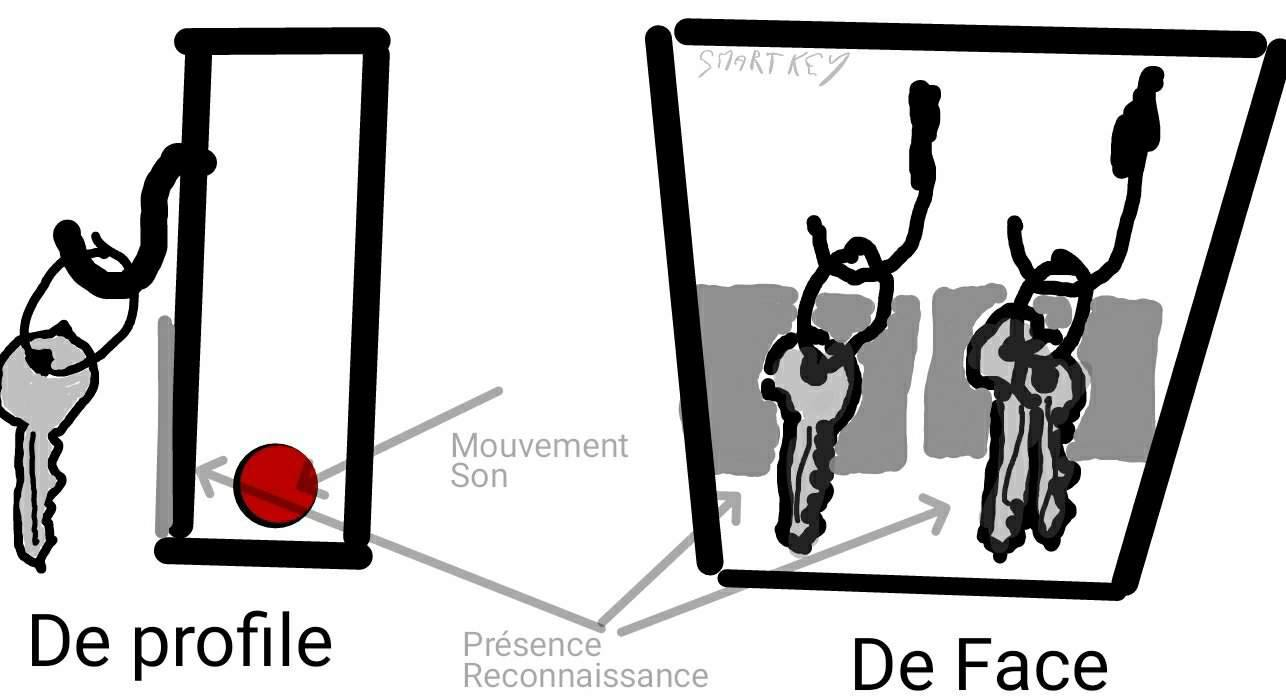
\includegraphics[scale=0.130]{Chroquis.jpg} 

\end{document}